\documentclass{article}
\usepackage[a4paper,margin=2.5cm]{geometry}
\usepackage{tikz}
\usetikzlibrary{arrows.meta,calc,positioning,backgrounds}
\pgfdeclarelayer{bg}
\pgfsetlayers{bg,main}
\usepackage{xcolor}
\usepackage{amsmath,amssymb}
\usepackage[english]{babel}
\usepackage[T1]{fontenc}
\usepackage[utf8]{inputenc}
\usepackage{lmodern}
\usepackage{upquote}
\usepackage{microtype}
\usepackage{parskip}
\usepackage{newunicodechar}
\newunicodechar{✓}{\ensuremath{\checkmark}}
\usepackage{longtable,booktabs,array}
\usepackage{calc} % for calculating minipage widths
% Correct order of tables after \paragraph or \subparagraph
\usepackage{etoolbox}
\makeatletter
\patchcmd\longtable{\par}{\if@noskipsec\mbox{}\fi\par}{}{}
\makeatother
% Allow footnotes in longtable head/foot
\IfFileExists{footnotehyper.sty}{\usepackage{footnotehyper}}{\usepackage{footnote}}
\makesavenoteenv{longtable}
\usepackage{enumitem}
\setlist{itemsep=0.2em, topsep=0.4em}
\usepackage{listings}
\lstset{
  basicstyle=\ttfamily\small,
  columns=fullflexible,
  breaklines=true,
  showstringspaces=false,
  upquote=true,
  literate={✓}{{$\\checkmark$}}1
}
\usepackage{xurl}
\usepackage[hidelinks]{hyperref}
\usepackage{bookmark}
\setlength{\emergencystretch}{3em} % prevent overfull lines
\setcounter{secnumdepth}{2} % automatic numbering for sections/subsections

\title{Real-Time Finance: Batch NBP Rates + Crypto Trade Stream}
\author{Adam Kaniasty, Igor Ko{\l}odziej}
\date{January 2026}

\begin{document}

\maketitle
\clearpage

{
\setcounter{tocdepth}{3}
\tableofcontents
}
\clearpage
\section{Project goal and scope}

The primary goal of the project is to build a complete batch-and-streaming
Big Data pipeline that combines daily FX rates published by the National
Bank of Poland (NBP) with a live market data stream from the Binance
exchange (final configuration: the BTCUSDT pair). The system should
support both bulk loading and historical analysis (batch layer) and the
creation of aggregated facts for fast reads in the serving layer.

The project uses a classic Big Data stack: Apache NiFi orchestrates data
flows and integrates external APIs, Apache Kafka serves as an optional
intermediate buffer, Apache HDFS is the main storage layer (raw/curated/
aggregated), Apache Spark performs ETL and batch analytics, Apache Hive
acts as a catalog and SQL layer over Parquet data, and Apache HBase is the
serving database. The entire stack runs in a Docker/Docker Compose
environment.

Functionally, the system implements multiple processing levels. The
curated layer produces two structured tables: \texttt{fx\_daily} (daily
NBP rates) and \texttt{trades\_agg\_hourly} (hourly crypto aggregates).
On top of these, Spark computes daily returns, daily and monthly
aggregated views, and a 63-day rolling correlation between BTC and the
USD/PLN exchange rate. The most important facts (e.g., closing prices,
volumes, and, with longer history, returns and correlations) are
published to the \texttt{finance:facts\_daily} table in HBase, enabling
fast reads by symbol and date.

Repeatability and ease of reproduction were key design requirements. All
steps -- from HDFS directory initialization, through Spark jobs, Hive
schema setup, to loading facts into HBase -- are wrapped in shell
scripts. An additional end-to-end script
(\path{tests/service/test-full-pipeline.sh}) runs the entire pipeline for
a given date and provides a simple way to demonstrate the solution.

\section{Data sources and their characteristics}

Below we summarize key parameters of the data sources used in the
project. The counts are shown for the reference run on
\texttt{2026-01-05} (for the crypto stream, the counts depend on the
length of the NiFi collection window).

{\small
\setlength{\tabcolsep}{2pt}
\renewcommand{\arraystretch}{1.0}
\begin{longtable}[]{@{}
  >{\raggedright\arraybackslash}p{(\linewidth - 12\tabcolsep) * \real{0.142}}
  >{\raggedright\arraybackslash}p{(\linewidth - 12\tabcolsep) * \real{0.142}}
  >{\raggedright\arraybackslash}p{(\linewidth - 12\tabcolsep) * \real{0.142}}
  >{\raggedright\arraybackslash}p{(\linewidth - 12\tabcolsep) * \real{0.142}}
  >{\raggedright\arraybackslash}p{(\linewidth - 12\tabcolsep) * \real{0.142}}
  >{\raggedright\arraybackslash}p{(\linewidth - 12\tabcolsep) * \real{0.142}}
  >{\raggedright\arraybackslash}p{(\linewidth - 12\tabcolsep) * \real{0.142}}@{}}
\toprule\noalign{}
\begin{minipage}[b]{\linewidth}\raggedright
Source
\end{minipage} & \begin{minipage}[b]{\linewidth}\raggedright
Type
\end{minipage} & \begin{minipage}[b]{\linewidth}\raggedright
Raw layer (HDFS)
\end{minipage} & \begin{minipage}[b]{\linewidth}\raggedright
Format
\end{minipage} & \begin{minipage}[b]{\linewidth}\raggedright
Ingestion frequency
\end{minipage} & \begin{minipage}[b]{\linewidth}\raggedright
Attributes (selected)
\end{minipage} & \begin{minipage}[b]{\linewidth}\raggedright
Row count (sample)
\end{minipage} \\
\midrule\noalign{}
\endhead
\bottomrule\noalign{}
\endlastfoot
Binance WebSocket (aggTrade) for BTCUSDT & streaming &
\path{/data/finance/raw/crypto-trades/date=YYYY-MM-DD/hour=HH/*.csv} &
JSON \textrightarrow{} CSV & continuous stream & \texttt{symbol},
\texttt{price}, \texttt{quantity}, \texttt{event\_time} &
\texttt{2026-01-05}: 24 CSV files, 781 event records
(\texttt{aggTrade}) \\
NBP API (Table A -- average rates) & batch (daily) &
\path{/data/finance/raw/nbp/date=YYYY-MM-DD/nbp_rate_{CODE}_{YYYYMMDD}.json}
& JSON & once per day (business days) & \texttt{code}, \texttt{currency},
\texttt{mid} (+ rate date) & \texttt{2026-01-05}: 32 files/records for
currencies (count depends on table/day) \\
\end{longtable}
}

For the same data sample, the processed layers (curated/aggregated) can
be verified with simple SQL queries against Hive tables (e.g.,
\texttt{SELECT} \texttt{...} \texttt{LIMIT} \texttt{5}; when needed,
\texttt{COUNT(*)}, although it is more expensive). Logs and sample
outputs from end-to-end runs are stored under
\path{artifacts/evidence_DATA_TIMESTAMP/}, generated by
\path{./tests/service/capture-evidence.sh}. Reference run example:
\path{artifacts/evidence_2026-01-05_20260106_100653/} (e.g.,
\texttt{pipeline.log}, \texttt{hive\_checks.log},
\texttt{hbase\_checks.log}).

To unambiguously verify data for a given date in Hive, we use date
filters (the column \texttt{`date`} is a Hive keyword and must be
escaped). Example checks for the reference run \texttt{2026-01-05}:

\begin{lstlisting}
SELECT count(*) AS fx_daily_rows FROM finance.fx_daily WHERE fx_date='2026-01-05'; -- 32
SELECT count(*) AS trades_rows FROM finance.trades_agg_hourly WHERE `date`='2026-01-05'; -- 2
SELECT count(*) AS crypto_daily_rows FROM finance.crypto_daily WHERE `date`='2026-01-05'; -- 1
SELECT * FROM finance.corr_btc_usdpln_63d WHERE `date`='2026-01-05'; -- NULL (no 63-day history)
\end{lstlisting}

Note that in a demo environment the crypto stream is typically collected
only for a short window within a single day, so history-dependent columns
(\texttt{ret\_1d}, 63-day correlation) may remain NULL. This behavior is
expected and consistent with the metric definitions.

\subsection{Streaming data -- Binance}

Our primary streaming source is the public Binance \texttt{aggTrade}
transaction stream for the BTCUSDT pair. Unlike the 24-hour ticker
stream, \texttt{aggTrade} carries actual trade events (price + quantity +
trade time), which makes batch aggregates (volume, trade count, OHLC)
semantically correct.

On the NiFi side, Binance data arrives as JSON through a WebSocket
processor and is validated and normalized into a strict record schema.
Depending on the variant, records are either grouped with
\texttt{MergeRecord} and written directly to HDFS, or buffered in Kafka
via \texttt{PublishKafkaRecord} and \texttt{ConsumeKafkaRecord}. In the
raw layer, HDFS stores CSV files under
\path{/data/finance/raw/crypto-trades/date=<YYYY-MM-DD>/hour=<HH>/...},
partitioned by date and hour. Each file contains a series of records
(CSV with header) with fields such as \texttt{symbol}, \texttt{price},
\texttt{quantity}, and \texttt{event\_time}.

The stream is potentially continuous, but in lab conditions the pipeline
runs in time windows of several to a dozen minutes. To reduce resource
usage, the final configuration ingests only BTCUSDT. After ETL, the
\texttt{trades\_agg\_hourly} table retains one aggregated observation per
(symbol, date, hour), which serves as the base for downstream analysis.

\subsection{Batch data -- NBP}

The second core data source is the public NBP API, which provides daily
exchange rate tables (the project uses Table A -- average rates). NiFi
periodically calls the HTTP endpoint for the latest rates table and then
splits it into individual records for each currency.

Each NBP record has a simple JSON structure: \texttt{currency} (currency
name), \texttt{code} (three-letter code, e.g., USD, EUR), and
\texttt{mid} (average rate versus PLN). NiFi also adds a date attribute
based on API response metadata. Files are written to HDFS under
\path{/data/finance/raw/nbp/date=<YYYY-MM-DD>/} as individual JSON files
per currency and day, e.g., \texttt{nbp\_rate\_USD\_20251204.json}.

The NBP API is updated once per day (business days), and a single
historical query is limited to 93 days. The architecture plan considered
windowed historical downloads (\(\le 93\) days), but the current
implementation focuses on daily ingestion of the latest tables and their
persistence in HDFS. A typical table contains several dozen currencies,
so a single date produces dozens of JSON files in the raw layer; after
processing, \texttt{fx\_daily} contains one observation per (date,
currency code).

\subsection{Optional sources (Kraken, Stooq)}

In the original project plan we considered extending the system with
additional sources: a transaction stream from Kraken (as a fallback in
case of Binance connectivity issues) and historical stock index quotes
from Stooq (e.g., WIG, WIG20) in CSV/ZIP format. Due to time constraints
and to refine the primary FX--crypto path, we focused on the two key
sources (Binance + NBP) and left Kraken/Stooq integration as a potential
future enhancement, to be listed in the "Future work" section.

\section{System architecture and tools}

The architecture is based on a clear layering model that separates
responsibilities for ingest, durable storage, batch processing/ETL, SQL
access, and publication of aggregated facts to a NoSQL serving layer. The
core is an HDFS cluster with three logical data tiers: raw, curated, and
aggregated. Each tier has a fixed directory structure described in the
documentation and initialization scripts
(\path{hdfs/create-directories.sh}).

\begin{figure}[htbp]
\centering
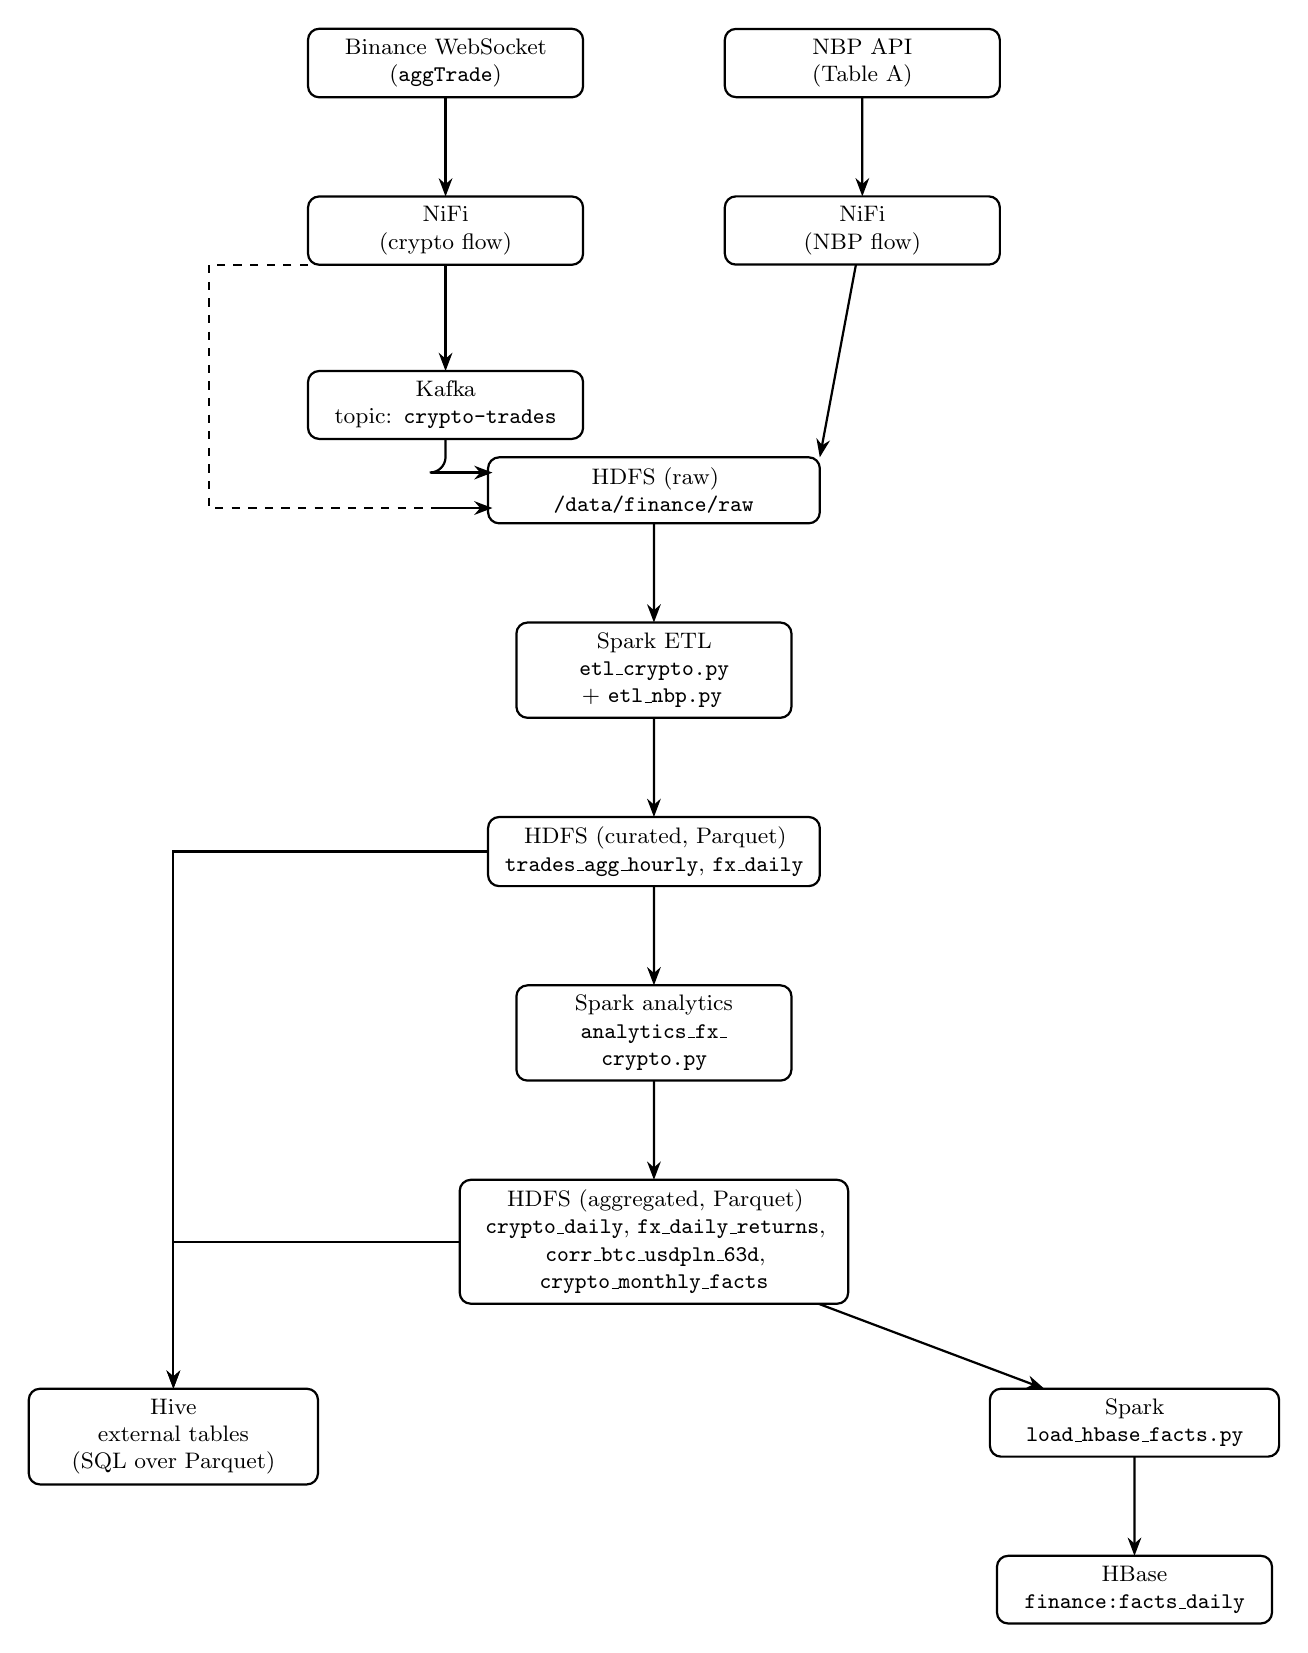
\begin{tikzpicture}[
  node distance=1.4cm and 2.0cm,
  scale=0.9, transform shape,
  >=Stealth,
  line cap=round,
  line join=round,
  every node/.style={font=\small},
  box/.style={draw, thick, rounded corners, fill=white, align=center, minimum height=9mm, inner sep=4pt, outer sep=0pt, text width=3.6cm},
  arrow/.style={->, thick},
  darrow/.style={->, thick, dashed},
  dline/.style={thick, dashed},
  % Arrowhead drawn as a short top-layer segment: do not extend it left (prevents the "T" artefact at the elbow),
  % but slightly extend it into the target node border for crisp termination.
  arrowhead/.style={->, thick, line cap=butt, shorten <= 0pt, shorten >= -1.6pt}
]
  \node[box] (binance) {Binance WebSocket\\(\texttt{aggTrade})};
  \node[box, right=of binance] (nbp) {NBP API\\(Table A)};

  \node[box, below=of binance] (nifiCrypto) {NiFi\\(crypto flow)};
  \node[box, below=of nbp] (nifiNbp) {NiFi\\(NBP flow)};

  \node[box, below=1.5cm of nifiCrypto, text width=3.6cm] (kafka) {Kafka\\topic: \texttt{crypto-trades}};

  \node[box, below=3.2cm of $(nifiCrypto)!0.5!(nifiNbp)$, text width=4.4cm] (hdfsRaw) {HDFS (raw)\\\texttt{/data/finance/raw}};

  \node[box, below=of hdfsRaw] (sparkEtl) {Spark ETL\\\texttt{etl\_crypto.py} + \texttt{etl\_nbp.py}};
  \node[box, below=of sparkEtl, text width=4.4cm] (hdfsCurated) {HDFS (curated, Parquet)\\\texttt{trades\_agg\_hourly}, \texttt{fx\_daily}};
  \node[box, below=of hdfsCurated] (sparkAn) {Spark analytics\\\texttt{analytics\_fx\_}\\\texttt{crypto.py}};
  \node[box, below=of sparkAn, text width=5.2cm] (hdfsAgg) {HDFS (aggregated, Parquet)\\\texttt{crypto\_daily}, \texttt{fx\_daily\_returns},\\\texttt{corr\_btc\_usdpln\_63d}, \texttt{crypto\_monthly\_facts}};

  \node[box, below left=1.2cm and 2.0cm of hdfsAgg, text width=3.8cm] (hive) {Hive\\external tables\\(SQL over Parquet)};
  \node[box, below right=1.2cm and 2.0cm of hdfsAgg, text width=3.8cm] (loadHbase) {Spark\\\texttt{load\_hbase\_facts.py}};
  \node[box, below=of loadHbase] (hbase) {HBase\\\texttt{finance:facts\_daily}};

  % Entry points on the left edge of HDFS(raw).
  % Keep them close to the vertical mid-line so they stay on the straight edge (not the rounded corners).
  \coordinate (hdfsRawInKafka) at ($(hdfsRaw.west)+(0,2.5mm)$);
  \coordinate (hdfsRawInNoKafka) at ($(hdfsRaw.west)+(0,-2.5mm)$);
  \coordinate (hdfsRawKafkaApproach) at ($(hdfsRawInKafka)+(-8mm,0)$);
  \coordinate (kafkaElbow) at (kafka.south |- hdfsRawKafkaApproach);
  \coordinate (kafkaArcStart) at ($(kafkaElbow)+(0,2mm)$);

  \begin{pgfonlayer}{bg}
    \draw[arrow] (binance) -- (nifiCrypto);
    \draw[arrow] (nbp) -- (nifiNbp);

    \draw[arrow] (nifiCrypto) -- (kafka);
    % Direct path without Kafka (dashed), routed around Kafka to keep the diagram readable.
    \draw[dline] (nifiCrypto.south west) -- ++(-1.4cm,0) |- ($(hdfsRawInNoKafka)+(-8mm,0)$);
    % Path with Kafka: Use rounded corners and |- (vertical then horizontal) logic
    \draw[thick, rounded corners=2mm] (kafka.south) |- (hdfsRawKafkaApproach);
    \draw[arrow] (nifiNbp) -- (hdfsRaw.north east);

    \draw[arrow] (hdfsRaw) -- (sparkEtl);
    \draw[arrow] (sparkEtl) -- (hdfsCurated);
    \draw[arrow] (hdfsCurated) -- (sparkAn);
    \draw[arrow] (sparkAn) -- (hdfsAgg);

    \draw[arrow] (hdfsCurated.west) -| (hive.north);
    \draw[arrow] (hdfsAgg.west) -| (hive.north);
    \draw[arrow] (hdfsAgg) -- (loadHbase);
    \draw[arrow] (loadHbase) -- (hbase);
  \end{pgfonlayer}
  % Kafka->HDFS arrowhead: short segment so no arrow line appears inside the node.
  \draw[arrowhead] ($(hdfsRawInKafka)+(-8mm,0)$) -- (hdfsRawInKafka);
  % No-Kafka arrowhead (drawn on top; solid to avoid dash-phase gaps near the border).
  \draw[arrowhead] ($(hdfsRawInNoKafka)+(-8mm,0)$) -- (hdfsRawInNoKafka);
\end{tikzpicture}
\caption{Architecture and data flow (with/without Kafka variants).}
\label{fig:architektura}
\end{figure}

Ingest is handled by Apache NiFi, which connects to external sources
(Binance, NBP), performs basic validation and transformation, and writes
records to HDFS. In the extended variant, data passes through Apache
Kafka as an intermediate buffer that improves resilience to connection
issues. In both cases, the result is raw CSV/JSON files under
\path{/data/finance/raw/crypto-trades/...} and
\path{/data/finance/raw/nbp/...}.

The raw layer is processed by Apache Spark, invoked in batch via
\path{spark/run-etl.sh} and \path{spark/run-analytics.sh}. The first
script builds the curated layer: normalization, deduplication (for NBP),
partitioning (\path{year/month} for NBP and \path{date/hour} for crypto),
and writing Parquet tables (\texttt{fx\_daily},
\texttt{trades\_agg\_hourly}). The second Spark stage performs analytics
-- computing returns, correlations, and monthly metrics -- and writes
results under \path{/data/finance/aggregated/...}. An additional script
\path{spark/run-check-analytics.sh} performs business-level sanity checks
(returns range, positive prices, correlation range).

Apache Hive serves as a catalog layer over Parquet data in HDFS. The
scripts \path{hive/init-tables.sh} and \path{hive/init-views.sh} create
external tables in the \texttt{finance} database mapping:
\begin{itemize}
\item the curated layer: \texttt{fx\_daily}, \texttt{trades\_agg\_hourly},
\item the aggregated layer: \texttt{fx\_daily\_returns},
  \texttt{crypto\_daily};\\
  \texttt{corr\_btc\_usdpln\_63d} and \texttt{crypto\_monthly\_facts}.
\end{itemize}
This makes both ETL outputs and analytical results accessible via SQL,
facilitating manual exploration and ad-hoc queries.

The serving layer is implemented in Apache HBase. The
\texttt{finance:facts\_daily} table, initialized by
\path{hbase/init-hbase.sh}, stores selected daily facts in a format
optimized for fast key-based reads (symbol + date). Loading data from the
aggregated layer into HBase is performed by a Spark job
(\path{spark/load\_hbase\_facts.py}) invoked via
\path{hbase/load-facts.sh}. Each full pipeline run ends with a control
scan of the HBase table, automated in
\path{tests/service/test-full-pipeline.sh}.

The entire stack runs under Docker/Docker Compose, allowing the
configuration to be reproduced on different machines without manual
installation of each component. Key services (HDFS, Hive, Spark, NiFi,
Kafka, HBase) are defined as separate containers in
\texttt{docker-compose.yml}. Hive serves as a metadata and SQL layer over
Parquet data in HDFS and runs in Hive-on-MR (local MapReduce), which
supports aggregate queries (e.g., \texttt{SELECT} \texttt{COUNT(*)},
\texttt{GROUP} \texttt{BY}) for demonstrational data sizes. Regardless of
this, all ETL and batch analytics are implemented in Spark as intended by
the architecture.

\section{Data ingestion, processing, and storage}

\subsection{NiFi + Kafka \textrightarrow{} HDFS (raw layer)}

The raw layer is built exclusively by Apache NiFi and, in the extended
variant, Apache Kafka. For the crypto stream, the main NiFi flow connects
to the Binance WebSocket API (\texttt{aggTrade}), validates and
transforms incoming JSON messages into a normalized record format (e.g.,
\texttt{ValidateRecord}, \texttt{UpdateRecord}), and then either groups
records into minute batches (\texttt{MergeRecord}) and writes directly to
HDFS (basic variant), or publishes them to a Kafka topic
(\texttt{crypto-trades}), from which they are consumed and written to
HDFS (buffered variant). The reference configuration uses the Kafka
variant (backup \path{nifi/backups/crypto-flow-kafka-4.json}), which
fulfills the buffering requirement. In both cases, raw crypto data lands
under \path{/data/finance/raw/crypto-trades/date=<YYYY-MM-DD>/hour=<HH>/...}
and is stored as CSV with headers.

For NBP, we use a batch flow: NiFi pulls the rates table (NBP API, Table
A) via \texttt{InvokeHTTP}, extracts metadata and splits the rates array
into individual elements (\texttt{EvaluateJsonPath} +
\texttt{SplitJson}), maps fields (\texttt{code}, \texttt{currency},
\texttt{mid}), and writes each record as a JSON file to HDFS
(\texttt{PutHDFS (NBP)}) under
\path{/data/finance/raw/nbp/date=<YYYY-MM-DD>/} with names like
\texttt{nbp\_rate\_<CODE>\_<YYYYMMDD>.json}. Unlike the crypto stream, we
do not use a Kafka buffer for NBP -- the data is small and daily, so a
direct HDFS write is sufficient.

NiFi flows are designed to be safe on re-runs: HDFS writes use "replace"
mode, and pipeline idempotency is ensured by the ETL layer (partition
overwrite; for NBP, additional deduplication by date+code). The choice
between Kafka and non-Kafka variants affects only the crypto stream
(backups \path{nifi/backups/crypto-flow.json} and
\path{nifi/backups/crypto-flow-kafka-4.json}) and does not change the
final HDFS data structure.

\subsection{Spark ETL \textrightarrow{} HDFS (curated layer)}

The curated layer transforms raw CSV/JSON files from HDFS into consistent
Parquet tables (with deduplication for NBP) that can be used directly in
analysis and exposed via Hive. The ETL process is implemented in Apache
Spark and run via \path{./spark/run-etl.sh}, which invokes two jobs:
\texttt{etl\_nbp.py} (NBP) and \texttt{etl\_crypto.py} (Binance).

For NBP, \texttt{etl\_nbp.py} reads JSON files from
\path{/data/finance/raw/nbp/date=<DATA>/nbp_rate_???_*.json}
(matching any three-character currency code in the file name). The file
name contains the rate date in \texttt{YYYYMMDD} format, extracted via
regex and converted to DATE (\texttt{fx\_date}).
Key fields (\texttt{code}, \texttt{currency}, \texttt{mid}) are selected,
rates are cast to DOUBLE, \texttt{load\_ts} is added, and partitioning
fields \texttt{year} and \texttt{month} are derived from the date. A
second deduplication step by (date, currency code) prevents multiple
loads of the same table. The result is written as Parquet to
\path{/data/finance/curated/nbp/fx_daily} using "dynamic partition
overwrite". Because we partition by (\texttt{year}, \texttt{month}), a
single-date refresh overwrites the entire month partition; with longer
history, ETL should process full months or extend partitioning by day.

Similarly, \texttt{etl\_crypto.py} processes raw CSV files under
\path{/data/finance/raw/crypto-trades/date=<DATA>/hour=<HOUR>/*.csv}.
Spark reads data with headers, casts numeric fields (\texttt{price},
\texttt{quantity}) to DOUBLE, and converts \texttt{event\_time}
(milliseconds since epoch) into TIMESTAMP (\texttt{event\_ts}). Records
missing key fields are dropped, and \texttt{date} (calendar day),
\texttt{hour}, and \texttt{hour\_start\_ts} (hour start) are derived from
the timestamp. Aggregation at the (symbol, date, hour) level computes
\texttt{price\_avg}, approximate 95th percentile (\texttt{price\_p95}),
hourly high/low (\texttt{price\_high}, \texttt{price\_low}), base volume
(\texttt{volume\_base} = sum of quantity), quote volume
(\texttt{volume\_quote} = sum of \texttt{quantity * price}), trade count
(\texttt{trade\_count}, number of \texttt{aggTrade} events), and
open/close prices (\texttt{price\_open}, \texttt{price\_close}) using
\texttt{min\_by}/\texttt{max\_by} over event time. The earliest and latest
timestamps within the hour (\texttt{ts\_min}, \texttt{ts\_max}) and
\texttt{load\_ts} are also recorded.

Aggregated data is written as Parquet to
\path{/data/finance/curated/crypto/trades_agg_hourly}, partitioned by
\texttt{date} (STRING) and \texttt{hour} (INT). As with NBP ETL, we use
dynamic partition overwrite, so re-running ETL for a given date/hour
refreshes data rather than duplicating it. The output is two stable,
well-defined curated tables (\texttt{fx\_daily},
\texttt{trades\_agg\_hourly}) that serve as the single source of truth
for downstream analytics.

\subsection{Hive over the curated layer}

To enable SQL access to the curated layer and easier exploration from
client tools (e.g., Beeline), Hive external tables are defined over the
Parquet files in HDFS. Their definitions are in
\path{hive/init_tables.sql}, and database/table initialization is
automated by \path{./hive/init-tables.sh}.

Two core external tables are created in the \texttt{finance} database:

\begin{itemize}
\item
  \texttt{finance.fx\_daily} pointing to
  \path{/data/finance/curated/nbp/fx_daily}, with schema matching the NBP
  ETL output: \texttt{fx\_date} (DATE), \texttt{code} (STRING),
  \texttt{currency} (STRING), \texttt{mid} (DOUBLE),
  \texttt{load\_ts} (TIMESTAMP), and partitions \texttt{year} (INT) and
  \texttt{month} (INT).
\item
  \texttt{finance.trades\_agg\_hourly} pointing to
  \path{/data/finance/curated/crypto/trades_agg_hourly}. The schema
  includes \texttt{symbol} (STRING), timestamps (\texttt{hour\_start\_ts},
  \texttt{ts\_min}, \texttt{ts\_max}), price fields
  (\texttt{price\_open}, \texttt{price\_close}, \texttt{price\_high},
  \texttt{price\_low}, \texttt{price\_avg}, \texttt{price\_p95}), volume
  fields (\texttt{volume\_base}, \texttt{volume\_quote},
  \texttt{trade\_count}), \texttt{load\_ts}, and partitions
  \texttt{date} (STRING) and \texttt{hour} (INT).
\end{itemize}

After creating the tables, \texttt{init-tables.sh} runs
\texttt{MSCK REPAIR TABLE} for each one, which automatically discovers
existing partition directories in HDFS and registers them in the Hive
metastore. As a result, partitions created by Spark ETL become visible
in Hive without manual registration. Correctness and data access are
verified by simple queries such as
\texttt{SELECT * FROM finance.fx\_daily LIMIT 5} and
\texttt{SELECT * FROM finance.trades\_agg\_hourly LIMIT 5}, executed as
part of the evidence script \path{tests/service/capture-evidence.sh}
(file \texttt{hive\_checks.log}) or manually during verification. In
practice, Hive acts as a catalog layer over curated data, while all
expensive aggregation operations are delegated to Spark.

\section{Data analysis and batch views (Spark + Hive)}

\subsection{Daily views -- FX and crypto}

After building the curated layer, the next step is to compute daily views
that serve as the basis for further aggregation and correlation. These
operations are implemented in a single Spark job
(\path{spark/analytics_fx_crypto.py}) run via
\path{./spark/run-analytics.sh}. The script performs four analytical
steps; the first two produce the daily FX and crypto views.

For FX rates, we compute \texttt{fx\_daily\_returns}. Based on the curated
\texttt{fx\_daily} table (including \texttt{fx\_date}, \texttt{code},
\texttt{mid}), we define a window ordered by date within each currency
(\texttt{code}). We then compute the previous-day rate
(\texttt{lag(mid)}) and the daily return
\texttt{ret\_1d = mid / lag(mid) - 1}. The result is written to
\path{/data/finance/aggregated/daily/fx_daily_returns} as Parquet
partitioned by \texttt{year} and \texttt{month} derived from
\texttt{fx\_date}. For the first day in each currency series, the return
remains NULL.

For crypto data, an analogous daily view \texttt{crypto\_daily} is
computed from the hourly aggregates in \texttt{trades\_agg\_hourly}. The
first step is to determine the daily close \texttt{close} for each
(symbol, date) pair, defined as \texttt{price\_close} from the last hourly
observation on that day (by \texttt{ts\_max}). Then, as for FX, we compute
\texttt{ret\_1d = close / lag(close) - 1} within each symbol. The
\texttt{crypto\_daily} view is written to
\path{/data/finance/aggregated/daily/crypto_daily} and partitioned by
\texttt{symbol} to facilitate downstream grouping.

\subsection{FX--crypto correlations}

Using daily returns for FX and crypto, we compute a 63-day rolling
correlation between the BTC market and the USD/PLN exchange rate. From
\texttt{crypto\_daily} we select only \texttt{BTCUSDT}, and from
\texttt{fx\_daily\_returns} we select the \texttt{USD} currency code. The
series are joined by date (\texttt{date}/\texttt{fx\_date}) to build daily
return vectors \texttt{ret\_btc} and \texttt{ret\_usdpln} for common days.

The resulting dataset is processed with a 63-day rolling window (in
practice: 63 consecutive observations, \texttt{rowsBetween(-62, 0)}). For
each date, we compute sums and sum of squares for \texttt{x} and
\texttt{y}, along with the sum of \texttt{x*y}, and then compute the
standard Pearson correlation between \texttt{ret\_btc} and
\texttt{ret\_usdpln}. The resulting view \texttt{corr\_btc\_usdpln\_63d}
contains the date and correlation value and is stored under
\path{/data/finance/aggregated/daily/corr_btc_usdpln_63d}. For early days
with fewer than two observations, the correlation remains NULL -- a full
63-day horizon is needed for a stable interpretation.

\subsection{Monthly views}

The final aggregation level in Spark is the monthly view
\texttt{crypto\_monthly\_facts}, computed from \texttt{crypto\_daily}. For
each (symbol, year, month), we compute basic metrics describing the
instrument in that month: average daily return (\texttt{avg\_ret\_1d}),
volatility measured as the standard deviation of daily returns
(\texttt{vol\_ret}), the number of days with available returns
(\texttt{days\_ret}), and the last available closing price in the month
(\texttt{last\_close}).

\texttt{crypto\_monthly\_facts} is written as Parquet to
\path{/data/finance/aggregated/monthly/crypto_monthly_facts} and
partitioned by \texttt{symbol}. This format simplifies filtering and
joining with other sources (e.g., FX correlations) and is a natural input
for the serving layer if we choose to publish monthly facts instead of
daily.

\subsection{Hive over the aggregated layer}

As in the curated layer, a set of Hive external tables is defined over
aggregated data under \path{/data/finance/aggregated/...} to allow SQL
inspection. The definitions are in \path{hive/init_views.sql}, and the
creation and basic verification are handled by \path{./hive/init-views.sh}.

Four external tables are created in the \texttt{finance} database:

\begin{itemize}
\item
  \texttt{finance.fx\_daily\_returns} over
  \path{/data/finance/aggregated/daily/fx_daily_returns} (columns:
  \texttt{fx\_date}, \texttt{code}, \texttt{mid}, \texttt{ret\_1d} and
  partitions \texttt{year}, \texttt{month}),
\item
  \texttt{finance.crypto\_daily} over
  \path{/data/finance/aggregated/daily/crypto_daily} (columns:
  \texttt{date}, \texttt{ts\_max}, \texttt{close}, \texttt{ret\_1d} and
  partition \texttt{symbol}),
\item
  \texttt{finance.corr\_btc\_usdpln\_63d} over
  \path{/data/finance/aggregated/daily/corr_btc_usdpln_63d} (columns:
  \texttt{date}, \texttt{corr\_btc\_usdpln\_63d}),
\item
  \texttt{finance.crypto\_monthly\_facts} over
  \path{/data/finance/aggregated/monthly/crypto_monthly_facts} (columns:
  \texttt{year}, \texttt{month}, \texttt{avg\_ret\_1d}, \texttt{vol\_ret},
  \texttt{days\_ret}, \texttt{last\_close} and partition \texttt{symbol}).
\end{itemize}

After creation, \texttt{init-views.sh} runs \texttt{MSCK REPAIR TABLE} for
partitioned tables, which registers existing partitions in the Hive
metastore. It then runs simple verification queries
(\texttt{SELECT * FROM ... LIMIT 5}) for each table to confirm that the
analytical views are available and consistent with Spark outputs. This
makes the analytical layer visible both to Spark and to SQL tools via
Hive, while computation remains in Spark.

\subsection{Sanity checks and tests}

Because the project values not just running analytics but also validating
its reasonableness, we implemented an additional sanity check script for
the aggregated layer: \path{spark/check_analytics_sanity.py}, executed by
\path{./spark/run-check-analytics.sh}. The script reads all four
analytical views:
\begin{itemize}
\item \texttt{fx\_daily\_returns}
\item \texttt{crypto\_daily}
\item \texttt{corr\_btc\_usdpln\_63d}
\item \texttt{crypto\_monthly\_facts}
\end{itemize}
and performs a set of simple but effective quality checks.

Among other things, it verifies that each view contains a non-zero number
of rows (which in practice indicates that ETL and analytics ran
correctly), that daily and monthly returns are not absurdly large (e.g.,
\textbar ret\_1d\textbar{} \textgreater{} 10), that closing prices are
positive, and that volatility (\texttt{vol\_ret}) is non-negative. For the
correlation table it checks that values fall in the expected range
{[}-1, 1{]} (with a small numerical margin). If any check fails, the
script exits with an error and prints a corresponding message, enabling
quick identification of data or logic issues. Sanity checks are included
in the full end-to-end test
(\path{tests/service/test-full-pipeline.sh}), so every pipeline run ends
with an automatic validation of analytical outputs.

\section{Serving layer -- HBase}

The final pipeline layer is the serving layer implemented in Apache
HBase. Its purpose is to expose selected aggregated metrics in a
structure optimized for fast key-based access (instrument symbol + date),
which enables lightweight client applications, dashboards, or ad-hoc
analysis without rerunning Spark jobs.

The central element is the \texttt{finance:facts\_daily} table, created
and reset by \path{hbase/init-hbase.sh}. The table is in the
\texttt{finance} namespace, and the row key format is
\texttt{salt|symbol|yyyyMMdd}, e.g., \texttt{2|BTCUSDT|20260105}. The
\texttt{salt} prefix (digit 0--9) is computed as
\texttt{abs(hash(symbol,\ date))\ \%\ 10} to spread keys and reduce
potential hot regions. The second part is the Binance symbol (BTCUSDT),
and the third is the date in \texttt{yyyyMMdd} format.

The table has four column families: \texttt{metrics}, \texttt{price},
\texttt{volume}, and \texttt{correlation}. In the current version we
populate selected columns:

\begin{itemize}
\item
  in \texttt{price}, the daily close as \texttt{price:avg} (from
  \texttt{crypto\_daily}),
\item
  in \texttt{volume}, the daily base volume as \texttt{volume:sum} (sum of
  \texttt{quantity}) and trade count as \texttt{volume:count} (sum of
  \texttt{trade\_count} from \texttt{trades\_agg\_hourly}),
\item
  in \texttt{metrics}, the daily return as \texttt{metrics:ret\_1d} for
  days where the return is defined (from the second observation onward),
\item
  in \texttt{correlation}, the column
  \texttt{correlation:btc\_usdpln\_63d}, which can store the 63-day BTC
  correlation with USD/PLN for the corresponding dates.
\end{itemize}

Loading data into HBase is performed by a dedicated Spark job
\path{spark/load_hbase_facts.py}, run via \path{./hbase/load-facts.sh}.
The job reads aggregated views (daily crypto facts from
\texttt{crypto\_daily}, volumes from \texttt{trades\_agg\_hourly}, and,
when sufficient history is available, correlations from
\texttt{corr\_btc\_usdpln\_63d}), joins them by symbol and date, and then
builds row keys in the format described above. Spark generates HBase Shell
\texttt{put} commands and writes them to
\path{/data/finance/hbase/facts_daily_puts} in HDFS as a plain text file.

The \texttt{load-facts.sh} script first ensures the
\texttt{finance:facts\_daily} table exists (calling \texttt{init-hbase.sh}),
then runs the Spark job to generate \texttt{put} commands, and finally
streams them from HDFS into HBase Shell via
\texttt{hdfs dfs -cat ... | hbase shell}. This avoids direct Spark-HBase
API integration and relies on a simple text bridge. After loading, the
script performs a control scan:

\begin{lstlisting}
scan 'finance:facts_daily', {LIMIT => 10}
\end{lstlisting}

In a typical run for the reference date (e.g., \texttt{2026-01-05}), the
scan shows a row for BTCUSDT with populated \texttt{price:avg},
\texttt{volume:sum}, \texttt{volume:count}, and (for days with defined
returns) \texttt{metrics:ret\_1d}. This confirms correct data flow from
the raw layer (NiFi/HDFS), through Spark ETL and analytics, to the HBase
serving layer. Additional scripts \path{hbase/verify-hbase.sh} and
\path{hbase/test-hbase.sh} independently verify table structure,
\path{put/get/scan} operations, and correctness across column families.

\section{Functional tests}

The project emphasizes test coverage for all key pipeline components
(NiFi, Kafka, HDFS, Spark, Hive, HBase) via shell scripts. This allows
running both individual layer tests and full end-to-end tests, with
repeatable results documented in logs.

\subsection{Ingest layer tests -- NiFi + HDFS}

These tests verify that NiFi flows correctly write Binance and NBP data
into the appropriate HDFS directories. Specifically:

\begin{itemize}
\item
  \path{tests/service/test-crypto-trades.sh} \texttt{DATE} \texttt{[HOUR]}
  checks for the presence and contents of crypto CSV files in
  \path{/data/finance/raw/crypto-trades/date=DATE/hour=HOUR/}. If
  \texttt{HOUR} is not provided, the script automatically selects the
  latest available hour for the day. It prints the path, file list, and
  file contents (limited to the first lines). Example run:
\end{itemize}

\begin{lstlisting}
./tests/service/test-crypto-trades.sh 2026-01-05 12
\end{lstlisting}

Output snippet:

\begin{lstlisting}
Reading CSV files from HDFS:
Path: /data/finance/raw/crypto-trades/date=2026-01-05/hour=12/

Files in directory:
-rw-r--r--   3 nifi supergroup       1812 ... /crypto-trades/date=2026-01-05/hour=12/05-12-44.csv
...
\end{lstlisting}

which confirms that NiFi correctly writes CSV files to the expected
location and format.

\begin{itemize}
\item
  \path{tests/service/test-nbp-rates.sh} \texttt{DATE} similarly checks
  \path{/data/finance/raw/nbp/date=DATE/} and lists JSON files with NBP
  rates. Example run:
\end{itemize}

\begin{lstlisting}
./tests/service/test-nbp-rates.sh 2026-01-05
\end{lstlisting}

Output snippet:

\begin{lstlisting}
Reading NBP exchange rate files from HDFS:
Path: /data/finance/raw/nbp/date=2026-01-05/

Files in directory:
-rw-r--r--   3 nifi supergroup         59 ... /nbp_rate_USD_20260105.json
...
\end{lstlisting}

which confirms that NBP data is available in HDFS as individual JSON
files for each currency.

\subsection{Kafka tests}

The script \path{tests/service/test-kafka.sh} runs integration tests for
Kafka:

\begin{itemize}
\item
  creating and listing temporary topics,
\item
  producing a few messages and consuming them,
\item
  validating message contents,
\item
  checking broker reachability from the host (port 9092).
\end{itemize}

Example output snippet:

\begin{lstlisting}
Kafka Comprehensive Tests
...
✓ PASS: Create topic: test-topic-...
✓ PASS: Produce messages to topic
✓ PASS: Consume messages (found 4 messages)
✓ PASS: Message content verification
✓ PASS: External connectivity (port 9092 accessible)
...
Passed: 8
Failed: 0
All tests passed!
\end{lstlisting}

which confirms correct Kafka configuration and integration with the test
container.

\subsection{Spark ETL and analytics tests}

Spark ETL and analytics are tested on two levels:

\begin{itemize}
\item
  via the full pipeline test (see Section 7.5), which runs
  \path{./spark/run-etl.sh}, \path{./spark/run-analytics.sh}, and
  \path{./spark/run-check-analytics.sh},
\item
  via direct execution of analytics sanity checks:
\end{itemize}

\begin{lstlisting}
./spark/run-check-analytics.sh
\end{lstlisting}

The script validates counts and value ranges across the four analytical
views:
\begin{itemize}
\item \texttt{fx\_daily\_returns}
\item \texttt{crypto\_daily}
\item \texttt{corr\_btc\_usdpln\_63d}
\item \texttt{crypto\_monthly\_facts}
\end{itemize}
Summary log snippet:

\begin{lstlisting}
Running analytics sanity checks...
[check] fx_daily_returns rows: 131
[check] crypto_daily rows: 1
[check] corr_btc_usdpln_63d rows: 1
[check] crypto_monthly_facts rows: 1
[check] All analytics sanity checks passed.
Analytics sanity checks completed successfully.
\end{lstlisting}

which confirms that analytical views are non-empty and satisfy basic
quality constraints (e.g., no extreme returns, positive prices, and
correlations within expected bounds when available).

\subsection{Hive tests}

Hive tests are integrated into the initialization scripts:

\begin{itemize}
\item
  \path{./hive/init-tables.sh}:

  \begin{itemize}
    \item
    creates the \texttt{finance} database and external tables
    \texttt{fx\_daily} and \texttt{trades\_agg\_hourly},
  \item
    runs \texttt{MSCK REPAIR TABLE} for both tables,
  \item
    verifies table existence with \texttt{SHOW TABLES} and runs simple
    \texttt{SELECT ... LIMIT 5} queries.
  \end{itemize}
\item
  \path{./hive/init-views.sh}:

  \begin{itemize}
    \item
    creates external tables over analytical views:\\
    \texttt{fx\_daily\_returns}, \texttt{crypto\_daily},\\
    \texttt{corr\_btc\_usdpln\_63d}, \texttt{crypto\_monthly\_facts},
  \item
    runs \texttt{MSCK REPAIR TABLE} for partitioned tables,
  \item
    executes control \texttt{SELECT ... LIMIT 5} queries for each table
    in the \texttt{finance} database.
  \end{itemize}
\end{itemize}

Running both scripts without errors and seeing the expected tables in
\texttt{SHOW TABLES IN finance} is treated as evidence of correct Hive
integration with curated and aggregated layers. Verification includes
built-in data samples (\texttt{SELECT ... LIMIT 5}); in this lightweight
stack, Hive-on-MR aggregates (e.g., \texttt{COUNT(*)}, \texttt{GROUP BY})
may work for demo-sized data but can be unreliable for heavier queries.
Nevertheless, all ETL logic and business analytics remain in Spark.

\subsection{HBase tests and end-to-end test}

The HBase layer has dedicated tests:

\begin{itemize}
\item
  \path{hbase/verify-hbase.sh}:

  \begin{itemize}
    \item
    checks HBase Shell availability,
  \item
    verifies the \texttt{finance} namespace and the
    \texttt{finance:facts\_daily} table,
  \item
    checks the presence of all column families (\texttt{metrics},
    \texttt{price}, \texttt{volume}, \texttt{correlation}),
  \item
    performs a test write/read of a sample row and then deletes it.
  \end{itemize}
\item
  \path{hbase/test-hbase.sh}:

  \begin{itemize}
    \item
    runs a series of write/read tests for multiple row keys,
  \item
    verifies access to individual column families,
  \item
    confirms table scanning capability.
  \end{itemize}
\end{itemize}

The most important test is the full end-to-end pipeline test
\path{tests/service/test-full-pipeline.sh} \texttt{YYYY-MM-DD}, which ties
all layers together. For the reference date \texttt{2026-01-05}, it
executes:

\begin{enumerate}
\def\labelenumi{\arabic{enumi}.}
\item
  \path{./spark/run-etl.sh} \texttt{--date} \texttt{2026-01-05} -- build the
  curated layer,
\item
  \path{./spark/run-analytics.sh} -- compute analytical views,
\item
  \path{./spark/run-check-analytics.sh} -- sanity checks,
\item
  \path{./hive/init-tables.sh} and \path{./hive/init-views.sh} -- initialize
  Hive tables,
\item
  \path{./hbase/load-facts.sh} \texttt{--date} \texttt{2026-01-05} -- publish
  facts to HBase.
\end{enumerate}

Final log snippet from a sample run:

\begin{lstlisting}
Step 3: Streaming commands from HDFS into HBase shell ...
...
Step 4: Verifying a few rows in HBase ...
scan 'finance:facts_daily', {LIMIT => 10}
ROW  COLUMN+CELL
 2|BTCUSDT|20260105 column=price:avg, ... value=92840.54
 2|BTCUSDT|20260105 column=volume:count, ... value=781
 2|BTCUSDT|20260105 column=volume:sum, ... value=19.974790000000013
1 row(s)
...
Full pipeline completed successfully for 2026-01-05
\end{lstlisting}

which unambiguously confirms that raw data (NiFi/HDFS) was correctly
processed by Spark ETL and analytics, registered in Hive, and finally
stored in HBase in the expected form. This test is the primary evidence
of system correctness and can be used as the key demonstration during
project presentation.

\section{Summary of the final solution}

In summary, the project delivered a complete, multi-layer Big Data
pipeline that meets the plan's goals: integrating batch NBP FX rates with
continuous Binance data, persisting them in HDFS, processing them in
Spark, exposing them via Hive, and publishing selected facts to HBase.
A key strength of the solution is that every step -- from HDFS directory
setup, through ETL and analytics, to Hive and HBase initialization -- is
scripted, enabling reproducible runs and easy demonstration
(\path{tests/service/test-full-pipeline.sh} runs the full pipeline for a
chosen date).

The most important design choices include a consistent layer structure
(raw/curated/aggregated/serving) with clear schema contracts and
idempotent Spark ETL (dynamic partition overwrite; NBP deduplication).
We also built analytical views aligned with business needs (returns,
correlations, monthly metrics) and designed the HBase key and schema for
fast access by symbol and date. An additional value is the sanity check
layer, which automatically validates the reasonableness of analytical
outputs and helps detect logic issues before results are published.

Several deliberate trade-offs were made. Due to the lack of a full YARN
environment, Hive runs in local MR mode and is used primarily as a
catalog and SQL layer over Parquet outputs (including simple aggregates
for demo data sizes). All meaningful transformations and analytics are
implemented in Spark, the primary processing engine. We also deferred
integration with additional sources (Kraken, Stooq) to focus on a robust
Binance + NBP pipeline. NiFi flow stability (e.g., behavior during
WebSocket disconnects) was validated manually during configuration and
testing.

It is also worth noting the final implementation decisions relative to
the plan. The aggregated view/table names in code and in this report do
not use the \texttt{v\_} prefix (e.g., \texttt{fx\_daily\_returns},
\texttt{corr\_btc\_usdpln\_63d}, \texttt{crypto\_monthly\_facts}), and the
raw crypto CSV includes the full aggTrade payload plus a normalized
subset of fields; the ETL layer uses only \texttt{symbol},
\texttt{price}, \texttt{quantity}, \texttt{event\_time}. In HBase we
ultimately populate \texttt{price:avg},
\texttt{volume:sum}, \texttt{volume:count}, \texttt{metrics:ret\_1d}, and
\texttt{correlation:btc\_usdpln\_63d}; the remaining metrics from the
plan (e.g., \texttt{vol\_21d}, additional price statistics) are a natural
future extension.

Potential future work includes extending the analytical layer with
additional metrics (e.g., 21-day volatility \texttt{vol\_21d}, other
correlation windows, risk indicators), adding automated scheduling for
ETL and analytics (e.g., cron or a dedicated orchestrator), integrating
with a visualization layer (dashboard over HBase), and expanding data
sources to additional exchanges or equity indices. The current version is
a solid foundation for these enhancements while meeting course
requirements and demonstrating a full end-to-end Big Data data flow.

\end{document}
